\section{Routing e Sicurezza}
\subsection{Routing Statico}
Il routing statico, anche denominato come instradamento statico, è un metodo che sfrutta percorsi prefissati dall’amministratore di rete. In questa maniera si può configurare un'intera rete molto velocemente, anche se con alcuni svantaggi. Infatti, il routing statico, avendo gli indirizzi fissi nelle varie macchine della rete, non è efficiente nella risoluzione di possibili errori. 

Il grande problema, infatti, si ha nel direzionare il pacchetto nella rete, se il percorso previsto per il pacchetto ha un errore al suo interno il traffico non viene ridirezionato e attende finché il percorso non sia stato riparato o finché l'amministratore di rete non abbia definito una nuova rotta. 

Nonostante ciò, però, il routing statico è ancora molto utilizzato e permette a piccole sottoreti interconnesse di lavorare al meglio e con pochi sforzi di gestione.

\subsubsection*{Configurazione computer con IP statici}
Per assegnare degli indirizzi IP in maniera statica ai dispositivi in una rete bastano 4 step, vediamone un esempio concreto svolto su CISCO packet tracer:

\begin{enumerate}
    \item Per prima cosa aprire la finestra relativa al dispositivo in questione (in questo caso un PC)\par
    \begin{sfigure}
        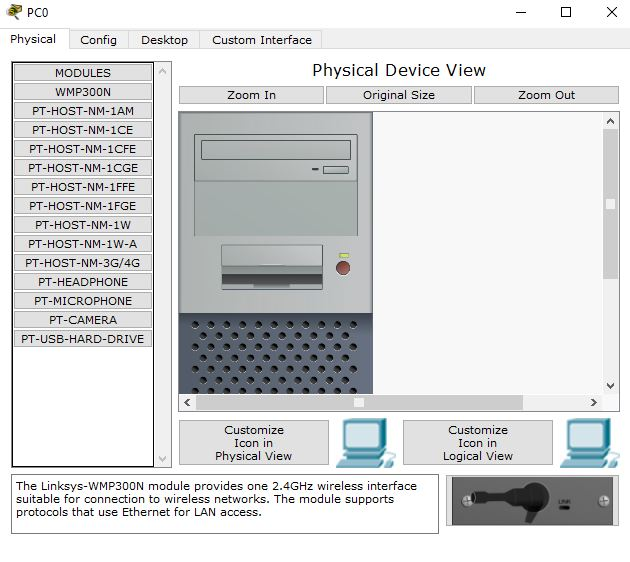
\includegraphics[width=0.6\linewidth]{images/07.routing-sicurezza/01.open-pc.jpg}
    \end{sfigure}
    \item Entrare nel Desktop del pc tramite il menu sovrastante\par
    \begin{sfigure}
        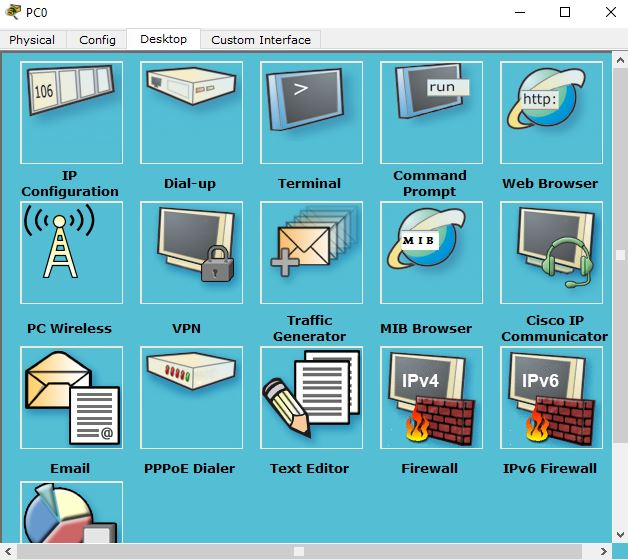
\includegraphics[width=0.6\linewidth]{images/07.routing-sicurezza/02.desktop-tab.jpg}
    \end{sfigure}
    \item Entrare nel menu della configurazione IP tramite l’icona presente nel desktop\par
    \begin{sfigure}
        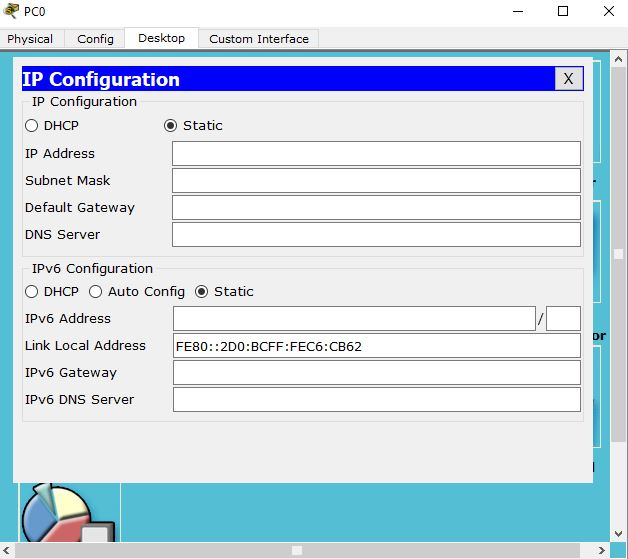
\includegraphics[width=0.6\linewidth]{images/07.routing-sicurezza/03.ip-config.jpg}
    \end{sfigure}
    \item In conclusione, inserire i dati riguardante gli indirizzi IP all’interno degli appositi come nell’esempio sotto riportato\par
    \begin{sfigure}
        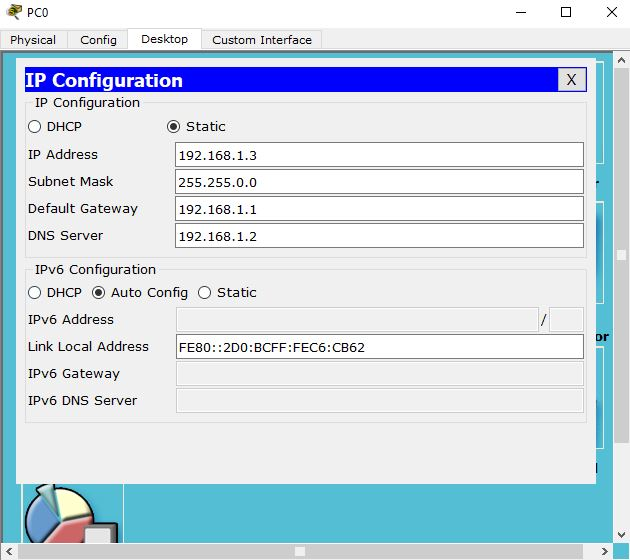
\includegraphics[width=0.6\linewidth]{images/07.routing-sicurezza/04.ip-config-complete.jpg}
    \end{sfigure}
\end{enumerate}

\subsubsection*{IP Route}
Il comando ip route è essenziale per la comunicazione tra reti a routing statico, dato che permette di creare rotte statiche e di conseguenza, instaurare il collegamento tra sottoreti. La sintassi del comando è molto semplice come vedremo a breve

Ecco come aggiungere una rotta tra router:

\begin{cmds}[Router]{Configuration mode}{cmd:ip-route-example}{Aggiungere una rotta statica nel router che indirizza i pacchetti destinati alla \textcolor{Highlight1}{rete specificata} verso l'\textcolor{Highlight2}{indirizzo IP o l'interfaccia} designata }
    \$ ip route \textcolor{Highlight1}{192.168.1.0 255.255.255.0} \textcolor{Highlight2}{172.16.100.1}
\end{cmds}

\subsection{VLAN}
Con il termine VLAN (Virtual Local Area Network) si intende la suddivisione di una rete locale, definita da uno switch, in più reti virtuali non comunicanti tra di loro ma appartenenti alla stessa infrastruttura fisica.

Per procedere alla suddivisione di una rete locale in più VLAN è necessario programmare lo switch a cui è associata la rete, quindi accedere alla console e digitare i seguenti comandi:

\begin{cmds}[Switch]{Configuration mode}{cmd:create-vlan}{Creare una VLAN in uno switch con \textcolor{Highlight1}{id} e \textcolor{Highlight2}{nome} arbitrario tuttavia la VLAN con ID 1 è utilizzata come default quindi convenzionalmente si utilizza la cifra delle decine (10, 20, ...)}
    \$ vlan \textcolor{Highlight1}{10}\\
    \$ name \textcolor{Highlight2}{sinistra}\\
    \$ vlan \textcolor{Highlight1}{20}\\
    \$ name \textcolor{Highlight2}{destra}
\end{cmds}

Una volta definite le VLAN si può procedere ad assegnare ad ogni rete virtuale le porte dello switch, suppondendo che lo switch abbia 24 porte in totali:

\begin{cmds}{Configuration mode}{cmd:setup-vlan-ports}{Configurazione delle porte dello switch modificando l'intero \textcolor{Highlight1}{range} di porte e assegnandole ad una \textcolor{Highlight2}{determinata VLAN}}
    \$ interface range \textcolor{Highlight1}{Fa 0/5-14}\\
    \$ switchport mode access\\
    \$ switchport access \textcolor{Highlight2}{vlan 10}\\
    \$ interface range \textcolor{Highlight1}{Fa 0/15-24}\\
    \$ switchport mode access\\
    \$ switchport access \textcolor{Highlight2}{vlan 20}
\end{cmds}

Un dettaglio importante di cui tenere conto quando si progettano le VLAN è quello di lasciare alcune porte non assegnate, così da poter definire eventuali porte di tronco. Una porta di tronco è una porta dello switch collegata ad un dispositivo esterno alle VLAN (come un router) e serve per permettere la comunicazione tra VLAN e i dispositivi collegati a quella porta.

Definizione di una porta di tronco:

\begin{cmds}[Switch]{Interfaccia esterna}{cmd:trunk-port}{Configurazione dell'interfaccia di tronco}
    \$ switchport mode trunk\\
    \$ switchport trunk allowed vlan
\end{cmds}

\subsection{VPN}
\subsection{Tunneling}
